\documentclass[tikz]{standalone}
\usetikzlibrary{shapes.geometric}    % trapezium
\usetikzlibrary{arrows}              % arrow tips
\usepackage{amsmath}
\usepackage{bm}                      % boldsymbol
\usepackage{makecell}                % makecell
\usetikzlibrary{matrix,calc}
\usepackage{color}
\usepackage{xcolor}
\definecolor{mygray}{HTML}{F0F0F0}
\usepackage{mathtools}
\usetikzlibrary{decorations.pathreplacing}
\begin{document}
    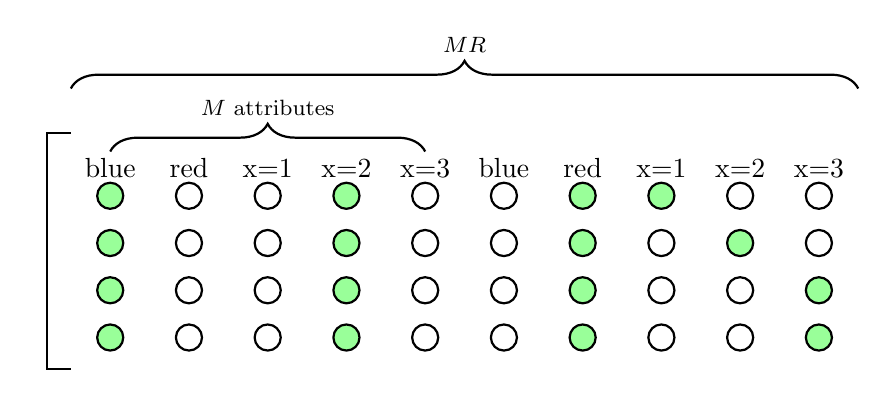
\begin{tikzpicture}[>=latex',thick]

      % matrix brackets
      \draw (-0.5, 0.8) --++(180:3mm)|-(-0.5,-2.2)
      node [pos=.25, above, rotate=90] {};



      % row
      \draw [decorate,decoration={brace,amplitude=10pt,raise=4pt},
      yshift=12pt] (-0.5,0.8) -- (9.5,0.8) node
      [black,midway,yshift=0.7cm] {\footnotesize $MR$};
      \draw [decorate,decoration={brace,amplitude=10pt,raise=4pt},
      yshift=12pt] (0,0) -- (4,0) node
      [black,midway,yshift=0.7cm] {\footnotesize $M$ attributes};

      % time 1
      \node [circle, draw=black, fill=green!40,
      label={[xshift=0, yshift=-0.08cm]blue}] at (0, 0) {};
      \node [circle, draw=black,
      label={[xshift=0, yshift=-0.08cm]red}] at (1, 0) {};
      \node [circle, draw=black,
      label={[xshift=0, yshift=-0.08cm]x=1}] at (2, 0) {};
      \node [circle, draw=black, fill=green!40,
      label={[xshift=0, yshift=-0.08cm]x=2}] at (3, 0) {};
      \node [circle, draw=black,
      label={[xshift=0, yshift=-0.08cm]x=3}] at (4, 0) {};
      \node [circle, draw=black,
      label={[xshift=0, yshift=-0.08cm]blue}] at (5, 0) {};
      \node [circle, draw=black, fill=green!40,
      label={[xshift=0, yshift=-0.08cm]red}] at (6, 0) {};
      \node [circle, draw=black, fill=green!40,
      label={[xshift=0, yshift=-0.08cm]x=1}] at (7, 0) {};
      \node [circle, draw=black,
      label={[xshift=0, yshift=-0.08cm]x=2}] at (8, 0) {};
      \node [circle, draw=black,
      label={[xshift=0, yshift=-0.08cm]x=3}] at (9, 0) {};

      % time 2
      \node [circle, draw=black, fill=green!40] at (0, -0.6) {};
      \node [circle, draw=black] at (1, -0.6) {};
      \node [circle, draw=black] at (2, -0.6) {};
      \node [circle, draw=black, fill=green!40] at (3, -0.6) {};
      \node [circle, draw=black] at (4, -0.6) {};
      \node [circle, draw=black] at (5, -0.6) {};
      \node [circle, draw=black, fill=green!40] at (6, -0.6) {};
      \node [circle, draw=black] at (7, -0.6) {};
      \node [circle, draw=black, fill=green!40] at (8, -0.6) {};
      \node [circle, draw=black] at (9, -0.6) {};

      % time 3
      \node [circle, draw=black, fill=green!40] at (0, -1.2) {};
      \node [circle, draw=black] at (1, -1.2) {};
      \node [circle, draw=black] at (2, -1.2) {};
      \node [circle, draw=black, fill=green!40] at (3, -1.2) {};
      \node [circle, draw=black] at (4, -1.2) {};
      \node [circle, draw=black] at (5, -1.2) {};
      \node [circle, draw=black, fill=green!40] at (6, -1.2) {};
      \node [circle, draw=black] at (7, -1.2) {};
      \node [circle, draw=black] at (8, -1.2) {};
      \node [circle, draw=black, fill=green!40] at (9, -1.2) {};

      % time 4
      \node [circle, draw=black, fill=green!40] at (0, -1.8) {};
      \node [circle, draw=black] at (1, -1.8) {};
      \node [circle, draw=black] at (2, -1.8) {};
      \node [circle, draw=black, fill=green!40] at (3, -1.8) {};
      \node [circle, draw=black] at (4, -1.8) {};
      \node [circle, draw=black] at (5, -1.8) {};
      \node [circle, draw=black, fill=green!40] at (6, -1.8) {};
      \node [circle, draw=black] at (7, -1.8) {};
      \node [circle, draw=black] at (8, -1.8) {};
      \node [circle, draw=black, fill=green!40] at (9, -1.8) {};



    \end{tikzpicture}
\end{document}